\documentclass[varwidth]{standalone}

\usepackage[]{graphicx}
\usepackage{subfigure}

\begin{document}
\begin{figure}
  \centering
	

  \hspace*{\fill}
  %\subfigure[]{\label{subfig:6a}\includegraphics[width=0.3\linewidth]{fig6a.png}} \hfill
  %\subfigure[]{\label{subfig:6b}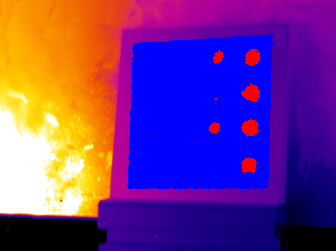
\includegraphics[width=0.3\linewidth]{fig6b.png}} 
  \subfigure[]{\label{subfig:6a}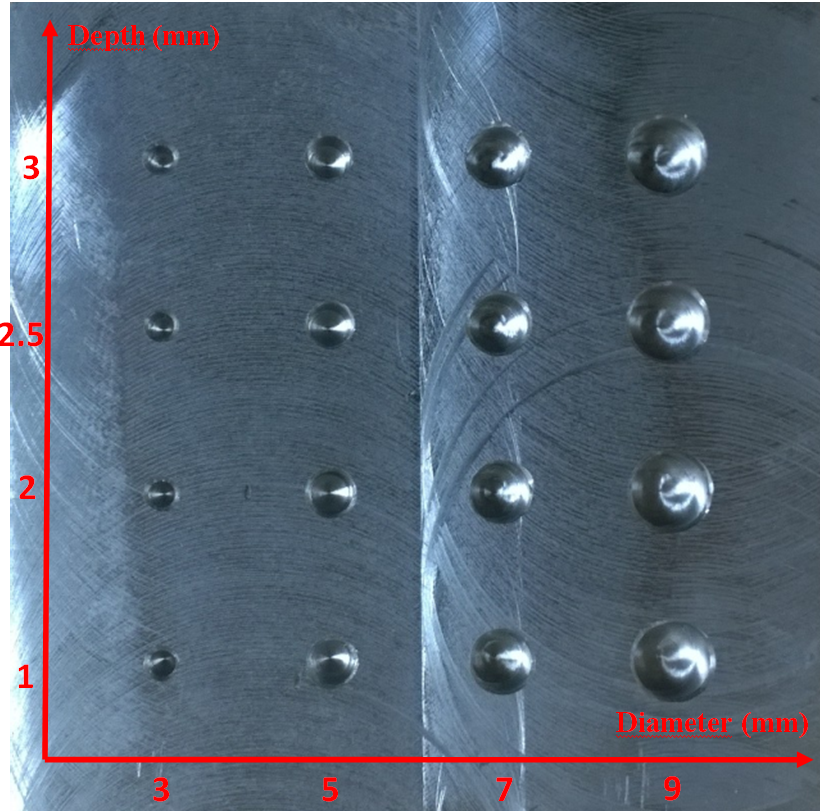
\includegraphics[width=0.3\linewidth]{fig7b.png}} \hfill
	\subfigure[]{\label{subfig:6b}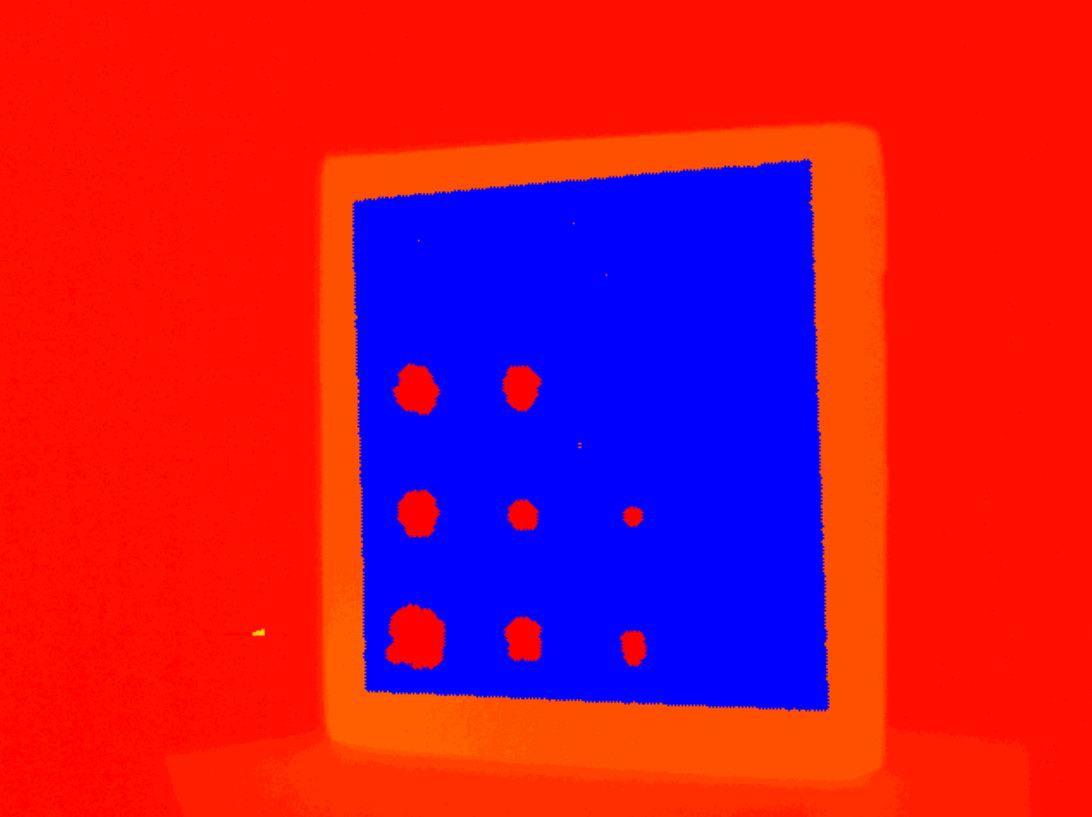
\includegraphics[width=0.3\linewidth]{fig7c.png}}
  \hspace*{\fill} \\ \hspace*{\fill}
  \subfigure[]{\label{subfig:6c}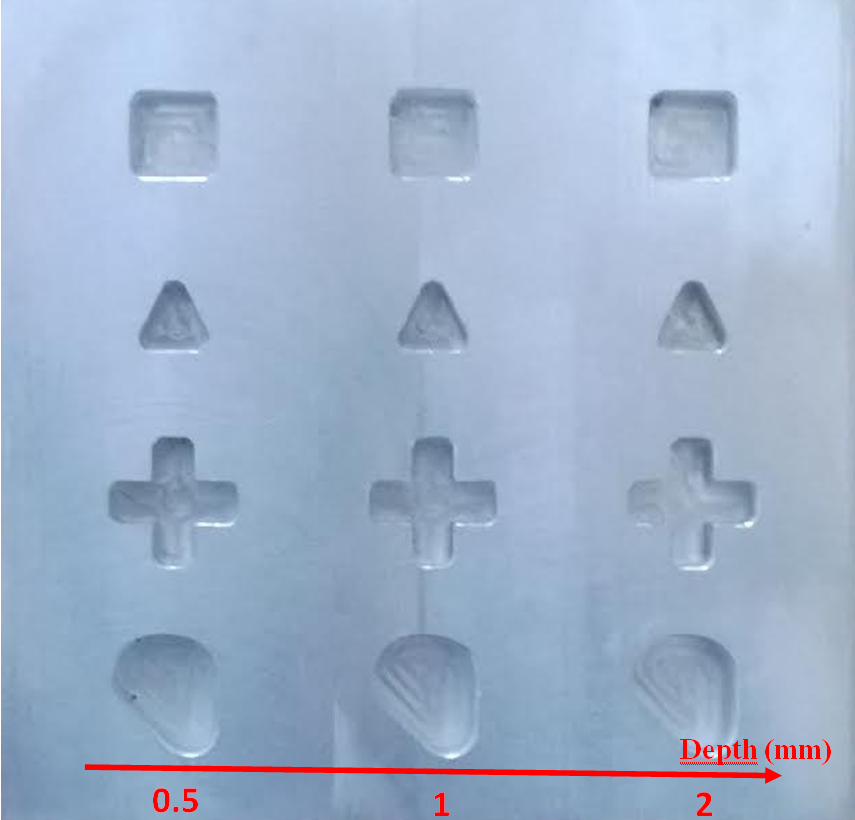
\includegraphics[width=0.3\linewidth]{fig6c.png}} \hfill
  \subfigure[]{\label{subfig:6d}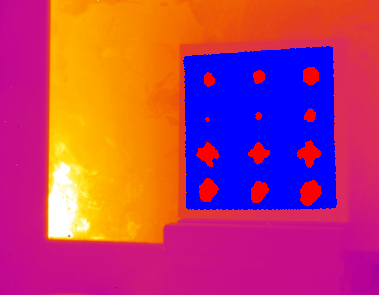
\includegraphics[width=0.3\linewidth]{fig6d.png}}
  \hspace*{\fill}
	
	  % \caption{(a) and (c) Steel and aluminum objects - (b) and (d) Corresponding detection map.}
		% \label{fig:6}
		\end{figure}
  \end{document}
